\documentclass[conference]{IEEEtran}
\IEEEoverridecommandlockouts
\usepackage{cite}
\usepackage{amsmath,amssymb,amsfonts}
\usepackage{algorithmic}
\usepackage{graphicx}
\usepackage{textcomp}
\usepackage{xcolor}

\begin{document}

\title{Spatially Distributed Multi-IMU Sensor Fusion via UKF for 6-DOF Rigid Body Kinematics}

\author{\IEEEauthorblockN{Berkay Nak}
\IEEEauthorblockA{\textit{Dept. of Electrical and Electronics Engineering} \\
\textit{Marmara University}\\
Istanbul, Turkey \\
150721016}
\and
\IEEEauthorblockN{\c{S}eref Keser}
\IEEEauthorblockA{\textit{Dept. of Electrical and Electronics Engineering} \\
\textit{Marmara University}\\
Istanbul, Turkey \\
150722019}
}

\maketitle

\begin{abstract}
This project investigates the feasibility of using low-cost Micro-Electromechanical Systems (MEMS) Inertial Measurement Units (IMUs) to build a responsive 6-Degree-of-Freedom (6-DOF) gyroscopic controller for human-computer interaction. A single MPU6500 IMU suffers from bias, high-frequency noise, and integration drift, therefore a spatially distributed array of three IMUs was used to obtain redundant angular-rate and acceleration measurements. First, a full-state Unscented Kalman Filter (UKF) was implemented offline to model the nonlinear rigid-body kinematics with quaternions, angular velocity, angular acceleration, and gyroscope bias. Then, a reduced-state online UKF-lite filter was implemented on the live serial stream to reduce sigma-point propagation cost and improve interaction latency. Experimental results show that the offline UKF provides smoother multi-sensor estimates than individual IMUs or raw averaging, while the online UKF-lite can track live hand motion with lower computational cost. The Normalized Innovation Squared (NIS) response also shows that abrupt human hand motions create non-Gaussian transients, which motivates a latency-oriented design for practical gyroscopic mouse applications.
\end{abstract}

\begin{IEEEkeywords}
Unscented Kalman Filter, Sensor Fusion, IMU, Quaternions, Human-Computer Interaction
\end{IEEEkeywords}

\section{Introduction}
The primary objective of this project is to build a highly responsive 6-DOF gyroscopic controller, also known as an air mouse. Raw measurements from low-cost MEMS IMUs such as the MPU6500 are not sufficient for precise cursor control when used directly. Gyroscope measurements contain bias and high-frequency noise, while accelerometer measurements are affected by both gravity and dynamic motion. These effects cause drift, jitter, and a heavy cursor feel when the measurements are integrated without filtering.

To improve observability without relying on expensive hardware, the controller was designed with three spatially distributed IMUs. The center, left, and right sensors measure the same rigid-body motion from different points on the device. This geometry creates redundant measurements and also exposes rotational effects through the lever-arm relationship between angular velocity, angular acceleration, and linear acceleration.

The resulting estimation problem is nonlinear because the device orientation evolves on the 3-D rotation manifold and because the acceleration measured at each IMU depends on cross-products of angular velocity and angular acceleration. An Extended Kalman Filter (EKF) could be used for this task, but it requires explicit Jacobian derivations. Instead, we used an Unscented Kalman Filter (UKF), which propagates deterministic sigma points through the nonlinear process and measurement models.

The project was implemented in two stages. The first stage used a full-state offline UKF to validate the multi-IMU rigid-body model on recorded data. The second stage used a reduced-state online UKF-lite filter driven by the live serial stream from the ESP32. This separation allowed us to compare model completeness against real-time responsiveness, which is the main trade-off in a human-computer interaction system.

\section{Mathematical Framework}

\subsection{Full-State Offline UKF}
For the offline analysis, spatial orientation is represented using a unit quaternion $\mathbf{q}$ to avoid gimbal lock. The full-state UKF tracks the kinematics at the controller's center of mass (COM):
\begin{equation}
\mathbf{x}_k =
\begin{bmatrix}
\mathbf{q}_k^T &
\boldsymbol{\omega}_k^T &
\boldsymbol{\alpha}_k^T &
\mathbf{b}_k^T
\end{bmatrix}^T
\in \mathbb{R}^{13},
\end{equation}
where $\mathbf{q}_k \in \mathbb{R}^4$ is the orientation quaternion, $\boldsymbol{\omega}_k \in \mathbb{R}^3$ is the angular velocity, $\boldsymbol{\alpha}_k \in \mathbb{R}^3$ is the angular acceleration, and $\mathbf{b}_k \in \mathbb{R}^3$ is the gyroscope bias.

The process model propagates the previous state over the sampling interval $\Delta t$:
\begin{equation}
\mathbf{x}_k = f(\mathbf{x}_{k-1}) + \mathbf{w}_{k-1},
\quad
\mathbf{w}_{k-1} \sim \mathcal{N}(0,Q).
\end{equation}
The quaternion is updated using the discrete-time quaternion derivative driven by angular velocity. The remaining states are modeled with slowly varying random-walk dynamics so that the filter can adapt to hand motion and sensor bias.

The measurement vector stacks the 6-axis measurements from the center, left, and right IMUs:
\begin{equation}
\mathbf{z}_k =
\begin{bmatrix}
\mathbf{z}_{c,k}^T &
\mathbf{z}_{l,k}^T &
\mathbf{z}_{r,k}^T
\end{bmatrix}^T
+ \mathbf{v}_k,
\quad
\mathbf{v}_k \sim \mathcal{N}(0,R).
\end{equation}
For an IMU located at displacement $\mathbf{r}_i$ from the COM, the rigid-body acceleration model is
\begin{equation}
\mathbf{a}_i =
\mathbf{a}_{com} +
\boldsymbol{\alpha}_k \times \mathbf{r}_i +
\boldsymbol{\omega}_k \times
\left(\boldsymbol{\omega}_k \times \mathbf{r}_i\right).
\end{equation}
This expression allows the offline UKF to use the spatial separation between IMUs rather than treating the sensors as three independent copies of the same measurement.

\subsection{Reduced-State Online UKF-Lite}
The full-state model is useful for analysis, but it is costly for a live mouse controller. A UKF with state dimension $n$ evaluates $2n+1$ sigma points at every update. Therefore, the 13-state offline filter requires 27 sigma-point propagations per sample, including the nonlinear quaternion and lever-arm measurement functions.

For the live serial implementation, the filter state was reduced to a compact state vector containing the angular-rate quantities required directly by the cursor pipeline:
\begin{equation}
\mathbf{x}^{lite}_k \in \mathbb{R}^{n_{lite}},
\quad n_{lite} < 13.
\end{equation}
The exact online state is intentionally smaller than the offline rigid-body state, so the number of sigma points decreases from 27 to $2n_{lite}+1$. The UKF-lite model avoids quaternion propagation inside the real-time control loop and prioritizes low latency and responsiveness, while the offline filter preserves a more complete rigid-body interpretation.

\section{Hardware and Data Acquisition}
The hardware platform consists of an ESP32 microcontroller and three MPU6500 IMUs placed at the center, left, and right positions of the controller body.

\subsection{Dual-I2C Architecture}
The MPU6500 supports two native I2C addresses, 0x68 and 0x69. To read three sensors without an external multiplexer, the ESP32's two hardware I2C buses were used. The center sensor at 0x68 and the left sensor at 0x69 share I2C0, while the right sensor at 0x68 operates on I2C1. Both buses operate in Fast Mode at 400 kHz.

\subsection{High-Speed Data Streaming}
The firmware runs on a 5 ms non-blocking timer and performs 200 Hz burst reads of the accelerometer, temperature, and gyroscope registers from all three IMUs. Raw measurements are scaled to physical units of $\mathrm{m/s^2}$ and $\mathrm{rad/s}$, then streamed to MATLAB through serial communication. The baud rate was set to 921600 bps to prevent the serial link from becoming the bottleneck. The same stream was used both for offline log analysis and for the online UKF-lite experiment.

\section{Experimental Results}

\subsection{Offline Multi-IMU Fusion}
The offline UKF was first evaluated on recorded multi-IMU motion data. Fig. \ref{fig_sensor_fusion} compares the individual gyroscope measurements, the raw average, and the UKF estimate. The individual IMUs show visible disagreement during fast motion segments because each sensor has its own noise, bias, and placement-dependent dynamics. Raw averaging reduces independent noise, but it cannot model the rigid-body constraints between spatially separated sensors. The UKF estimate remains smoother and more coherent during the main right-left, up-down, and roll motion intervals.

\begin{figure}[htbp]
\centerline{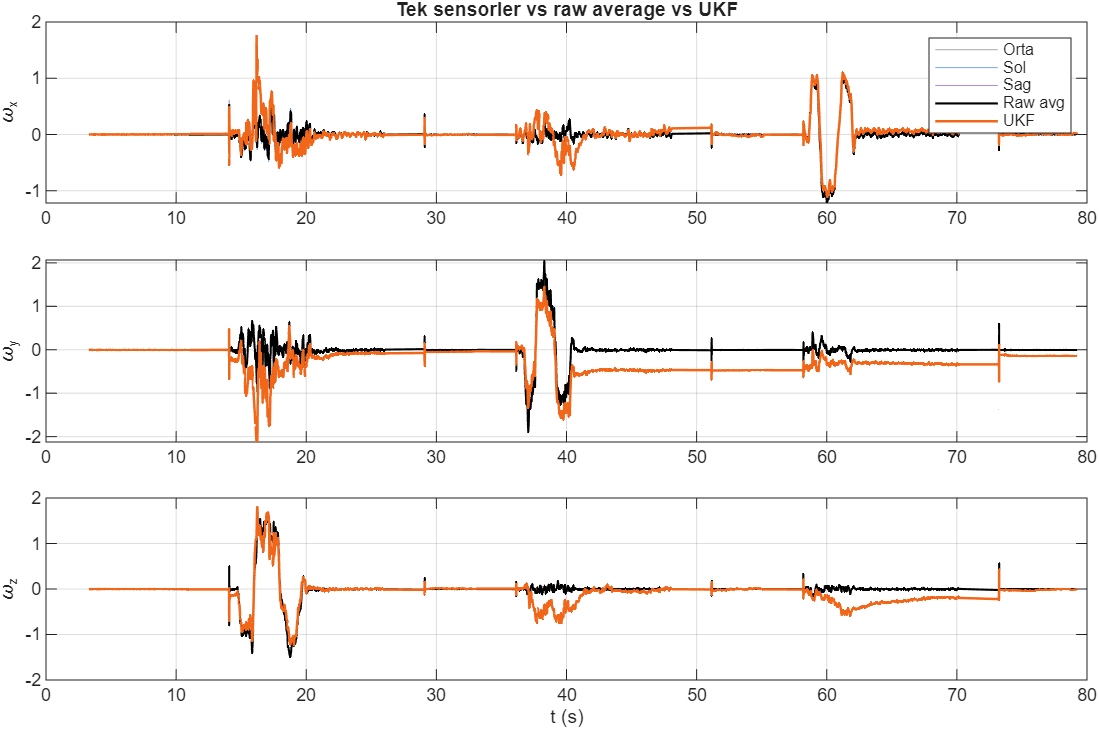
\includegraphics[width=\linewidth]{fig_sensor_fusion_comparison.png}}
\caption{Offline sensor fusion comparison between individual IMUs, raw gyroscope averaging, and the UKF estimate. The UKF reduces measurement jitter while preserving the dominant motion profile.}
\label{fig_sensor_fusion}
\end{figure}

Fig. \ref{fig_offline_velocity} shows the offline angular velocity estimates for the three rotational axes. The lower subplot shows the innovation magnitude. Innovation increases mainly during abrupt hand motion, where the measurement departs from the filter prediction. During lower-dynamic intervals, the UKF output remains close to zero and suppresses small raw fluctuations.

\begin{figure}[htbp]
\centerline{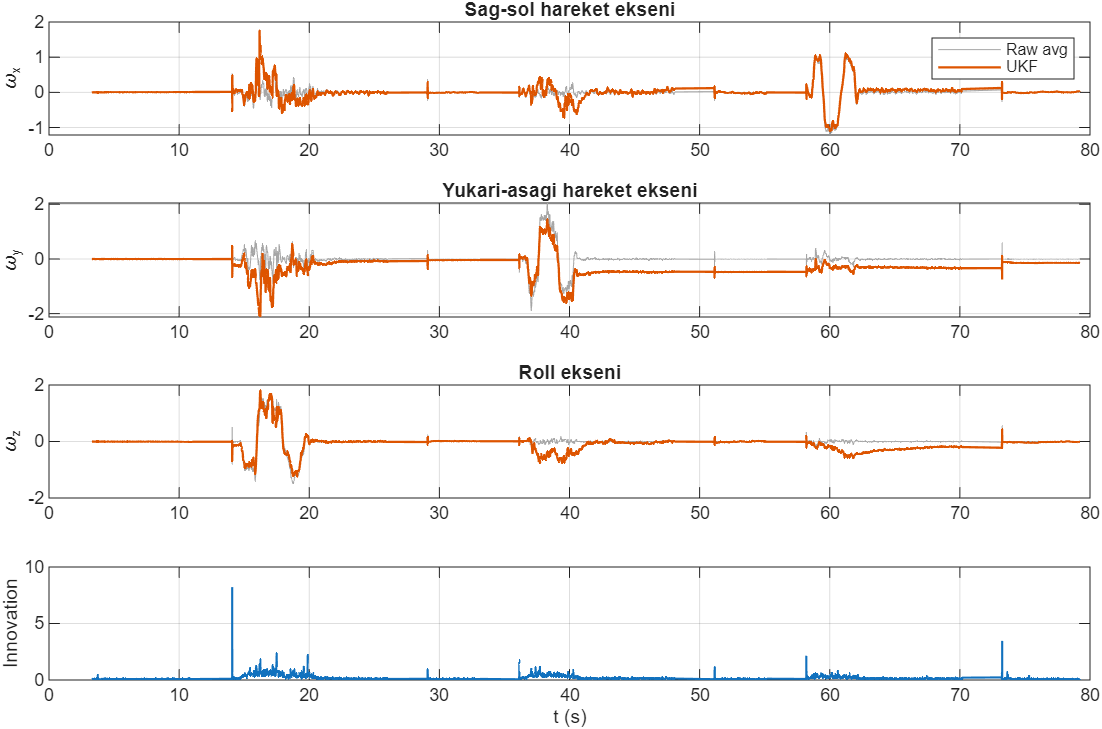
\includegraphics[width=\linewidth]{fig_offline_ukf_angular_velocity.png}}
\caption{Offline UKF angular velocity estimation for the right-left, up-down, and roll axes. The innovation signal rises during sudden motion and remains small during stationary intervals.}
\label{fig_offline_velocity}
\end{figure}

Because the offline filter includes angular acceleration in the state vector, it can also estimate $\boldsymbol{\alpha}$ directly. Fig. \ref{fig_offline_acceleration} shows that the acceleration estimate is concentrated around motion transitions and rapid direction changes. These peaks are expected because angular acceleration is most observable when the hand starts, stops, or reverses motion.

\begin{figure}[htbp]
\centerline{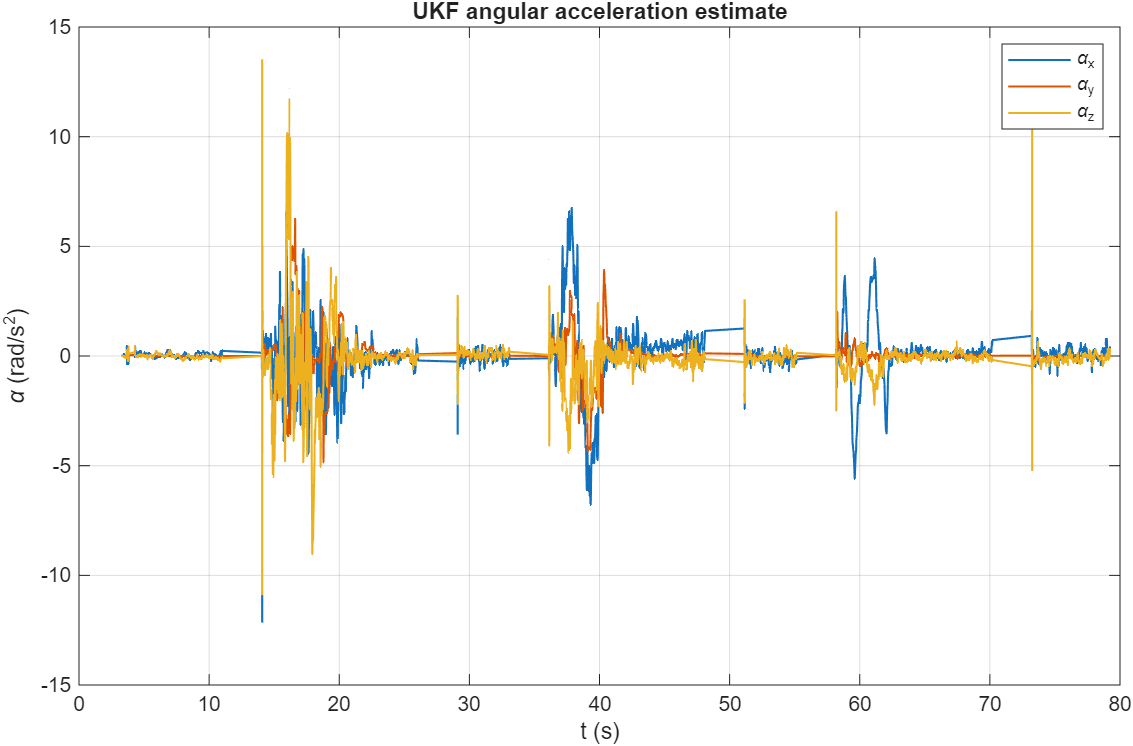
\includegraphics[width=\linewidth]{fig_offline_ukf_angular_acceleration.png}}
\caption{Offline full-state UKF angular acceleration estimate. Peaks occur at motion onsets, stops, and direction reversals, where rotational acceleration is physically strongest.}
\label{fig_offline_acceleration}
\end{figure}

\subsection{Consistency Analysis}
The Normalized Innovation Squared (NIS) was used to evaluate whether the measurement residuals are statistically consistent with the predicted innovation covariance:
\begin{equation}
\epsilon_k =
\boldsymbol{\nu}_k^T
S_k^{-1}
\boldsymbol{\nu}_k,
\end{equation}
where $\boldsymbol{\nu}_k$ is the innovation and $S_k$ is its covariance. For an ideally tuned Gaussian model, the NIS should remain near the expected measurement dimension except for statistically rare outliers.

The real recorded data in Fig. \ref{fig_nis} does not behave like an ideal Gaussian simulation. Most samples remain close to the expected region, but several large spikes occur during abrupt manual motion, with the largest spike appearing near the first strong excitation. These spikes indicate that sudden human hand movements, sensor saturation, or unmodeled placement effects can violate the assumed noise model. Therefore, the NIS result is useful not only as a consistency check, but also as evidence that a user-facing controller must be tuned for responsiveness rather than only statistical smoothness.

\begin{figure}[htbp]
\centerline{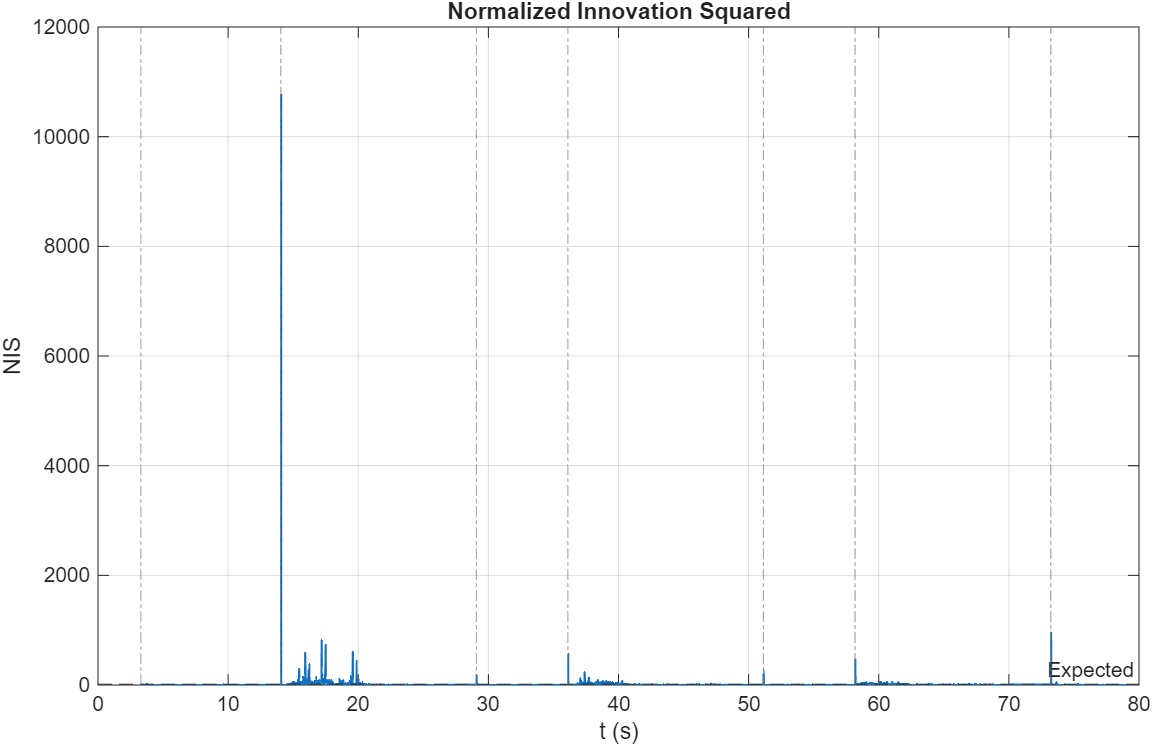
\includegraphics[width=\linewidth]{fig_ukf_consistency_nis.png}}
\caption{Offline UKF Normalized Innovation Squared (NIS). Large transient spikes occur during abrupt hand motion, revealing model mismatch under highly dynamic interaction.}
\label{fig_nis}
\end{figure}

\subsection{Live UKF-Lite Serial Experiment}
After validating the offline filter, a reduced-state UKF-lite was tested on the live serial stream. Fig. \ref{fig_live_lite} shows the online angular velocity estimates. The first three subplots correspond to right-left motion, up-down motion, and roll. The UKF-lite output follows the raw averaged gyroscope signal closely, which is desirable for an interactive mouse because excessive smoothing would be perceived as latency. The fourth subplot shows the online NIS diagnostic, where spikes again appear during aggressive hand motion.

\begin{figure}[htbp]
\centerline{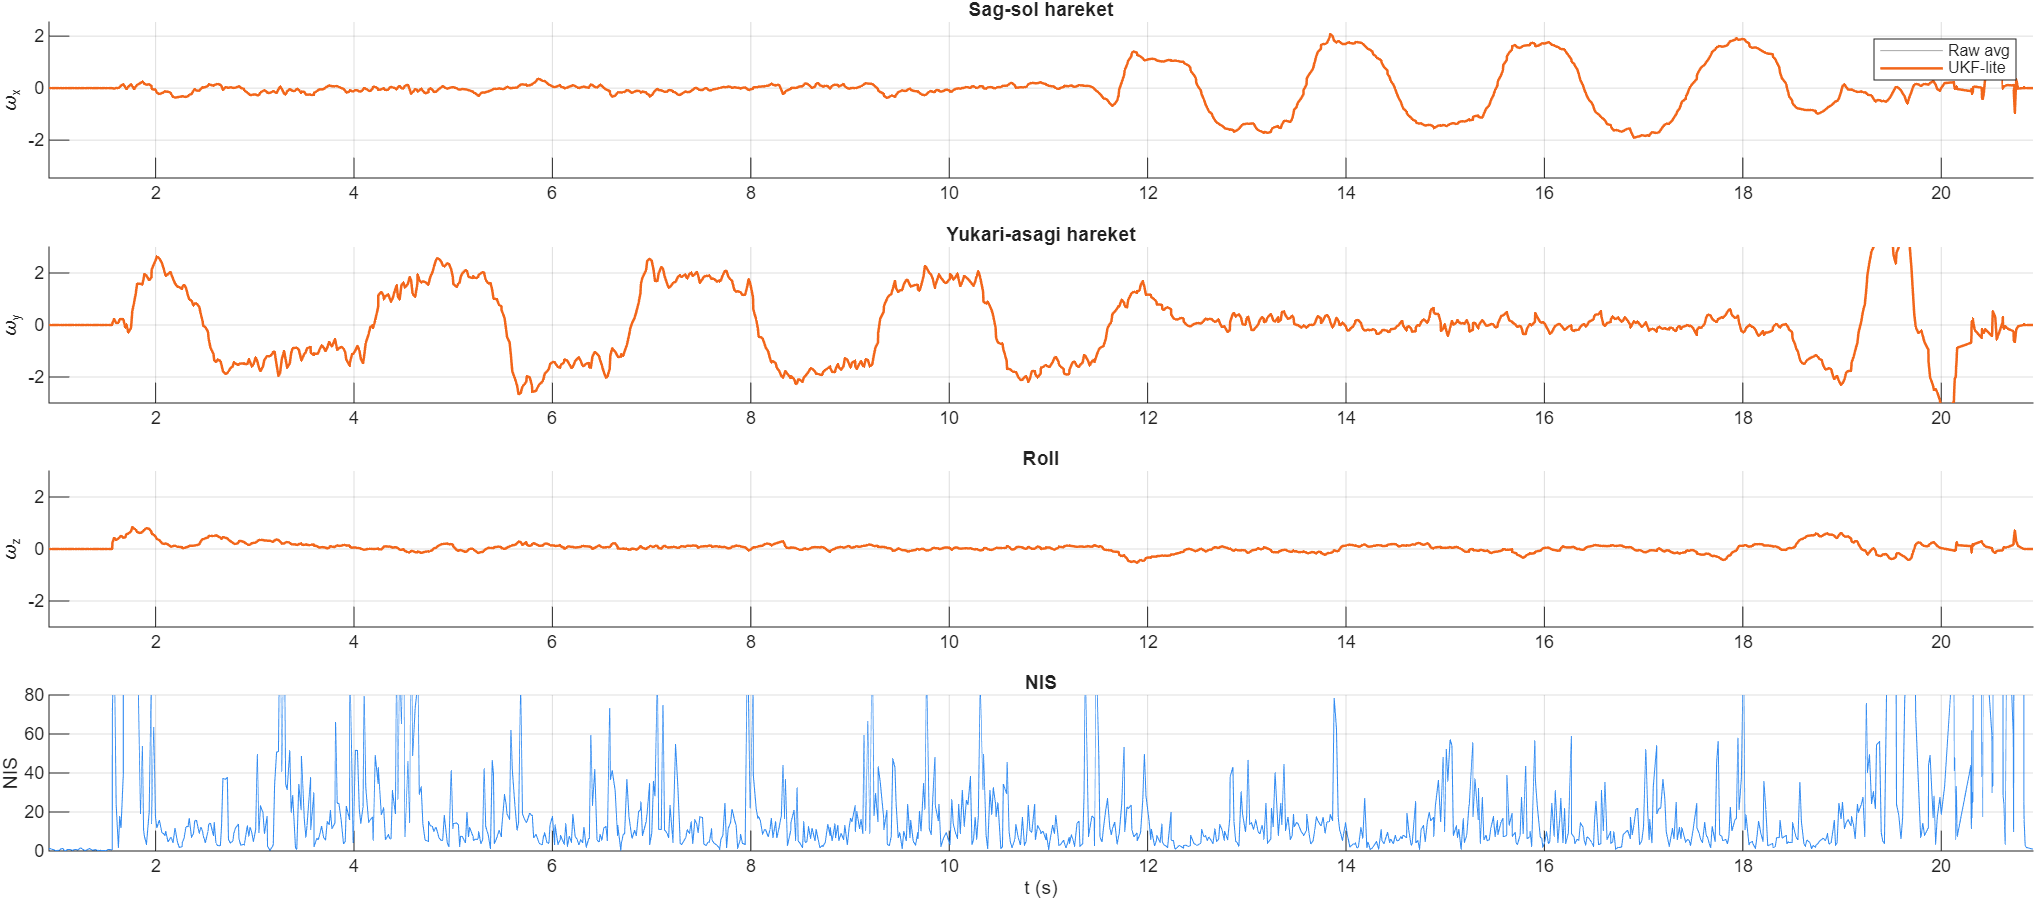
\includegraphics[width=\linewidth]{fig_live_ukf_lite_angular_velocity.png}}
\caption{Live reduced-state UKF-lite angular velocity estimation from the ESP32 serial stream. The reduced model tracks intentional hand motion with low latency while retaining NIS as an online diagnostic.}
\label{fig_live_lite}
\end{figure}

Compared with the offline full-state UKF, the live UKF-lite sacrifices angular acceleration and quaternion-state estimation inside the real-time loop. However, this reduction decreases the number of sigma points and avoids expensive nonlinear propagation at each 5 ms update. For a gyroscopic mouse, this trade-off is practical because the cursor primarily requires responsive angular-rate information rather than a complete offline reconstruction of the rigid-body state.

\section{Discussion and Conclusion}
The experiments show that a spatially distributed three-IMU structure improves the quality of low-cost inertial sensing. In offline analysis, the full-state UKF fuses the redundant measurements into smoother angular velocity estimates and also provides angular acceleration estimates that align with motion transitions. This confirms that the multi-IMU geometry contains useful rigid-body information beyond a simple single-sensor reading.

However, the live experiment also shows why the estimation strategy must be different for human-computer interaction. A full UKF is designed to produce statistically smooth state estimates, while an air mouse must respond immediately to intentional hand motion. Abrupt user inputs appear as innovation spikes, and aggressive filtering can make the cursor feel delayed or heavy. Therefore, the reduced-state UKF-lite is a better match for online operation because it tracks the angular velocity states required by the cursor while reducing computation and smoothing latency.

In conclusion, the full-state UKF is valuable as an offline modeling and validation tool for spatially distributed IMU fusion. For real-time gyroscopic mouse control, a reduced-state online filter provides a more practical balance between noise reduction and responsiveness. Future work should combine the online UKF-lite with deterministic multi-IMU algebraic features and complementary filtering so that the final controller can preserve low latency while still benefiting from the redundancy of the three-sensor array.

\section*{Acknowledgment}
The authors thank Prof. Dr. Engin Masazade for his guidance in EE4084. During the preparation of this work, the authors utilized ChatGPT to generate structural drafts and improve the wording of specific sections, including the Abstract, Results, Discussion, and Conclusion sections. Following the use of this tool, the authors thoroughly reviewed and edited the material, and assume full responsibility for the final content of the publication.

\end{document}
